% 第4章第2节（上）：矩阵的表示（矩阵、元素与形状，设计矩阵与贯穿例）、常见矩阵（方阵、零矩阵、对角矩阵、单位矩阵、上三角矩阵、下三角矩阵、对称矩阵、正定矩阵与半正定矩阵、置换矩阵、正交矩阵）、矩阵的运算（加法与数乘、转置、矩阵与向量的乘积、矩阵乘法、逐项乘积、逆矩阵、矩阵幂、迹、Frobenius内积、Frobenius范数、诱导矩阵范数、行列式）。运算的性质见03-matrix-properties.tex。

\section{矩阵}
\label{sec:ls-matrices}

一批样本的特征排成一张数表以后，问题随之而来：对每个样本用同一组权重求加权和，要算许多个同样形式的和，能否一次写出；两次这样的计算接连进行，能否合成一次；一次计算能否撤销，反复进行时怎样书写；一张表把单位正方形变成平行四边形时，面积放大多少；作为计算，它最多把输入放大多少倍。这些问题都以矩阵为对象。本节先规定矩阵的写法，再介绍元素分布有固定模式的几类常见矩阵，然后逐一定义矩阵的运算，最后按运算整理它们满足的性质。

与向量不同，矩阵最重要的运算不是逐项进行的加法，而是由加权求和导出的乘法。乘法的规则与实数乘法有同有异，需要逐条核对。

\subsection{矩阵的表示}
\label{sec:ls-matrix-representation}

定位向量中的一个数需要一个索引；一张数表的每个数要由所在的行与列共同确定，需要两个索引。

\paragraph{矩阵、元素与形状}
$m$行$d$列的实数表称为矩阵（matrix），记为$\bm A\in\mathbb R^{m\times d}$；第$i$行、第$j$列的元素记为$\bm A_{i,j}$，不会混淆时也写作$a_{i,j}$。$m\times d$称为矩阵的形状，行数写在列数之前。记号$\bm A_{i,:}$表示第$i$行，$\bm A_{:,j}$表示第$j$列，冒号表示该方向上的全部位置；第$j$列是一个$m$维列向量，第$i$行是一个$d$维行向量。例如在
\[
 \bm A=\begin{bmatrix}1&2&3\\4&5&6\end{bmatrix}\in\mathbb R^{2\times3}
\]
中，$\bm A_{2,1}=4$，第一行$\bm A_{1,:}=\left[\begin{smallmatrix}1&2&3\end{smallmatrix}\right]$，第三列$\bm A_{:,3}=(3,6)^\top$。

两个矩阵相等，要求形状相同且每个对应元素相等。只有一行的矩阵就是行向量，只有一列的矩阵就是列向量，所以向量可以看作矩阵的特例。

\paragraph{设计矩阵}
用矩阵记录数据时，通常让每行对应一个样本，每列对应一个特征，这样的矩阵称为设计矩阵。把示例~\ref{ex:ls-nearly-collinear-features}中两个特征的取值向量$\bm c_1,\bm c_2$并排作为两列，得到三个样本、两个特征的设计矩阵
\begin{equation}
 \bm X_{\varepsilon}
 =\begin{bmatrix}1&1\\1&1+\varepsilon\\1&1-\varepsilon\end{bmatrix}
 =\begin{bmatrix}\bm c_1&\bm c_2\end{bmatrix},
 \qquad
 \bm q=\begin{bmatrix}0\\1\\-1\end{bmatrix},
 \quad \bm c_2=\bm c_1+\varepsilon\bm q.
 \label{eq:linear-algebra-nearly-collinear-design}
\end{equation}
$|\varepsilon|$很小时，两列之差$\bm c_2-\bm c_1=\varepsilon\bm q$很短，两列几乎是同一串数；第~\ref{sec:ls-inner-product-definition}节将用夹角说明它们几乎同向。这个例子将贯穿整个线性空间部分：第~\ref{chap:linear-representation}章讨论这样两列能否充当一组记录方向，后续两章再看它怎样影响谱、求解与误差。

\subsection{常见矩阵}
\label{sec:prelim-common-matrices}

有些矩阵的元素分布有固定模式：大部分位置为零，或者主对角线两侧互相对称，或者各列彼此正交；对称矩阵中还有一类由二次型的符号刻画。这些模式会让后面的运算大为简化。本小节按元素的位置与取值逐类给出定义和例子；它们在乘法、转置、求逆下怎样表现，放到第~\ref{sec:ls-matrix-operation-properties}节讨论。

\paragraph{方阵}
行数等于列数的矩阵称为方阵（square matrix），$n\times n$方阵也称$n$阶方阵；位置$(i,i)$上的元素组成主对角线。例如$\left[\begin{smallmatrix}1&2\\3&4\end{smallmatrix}\right]$是二阶方阵，主对角元素为$1$和$4$；$2\times3$矩阵不是方阵，也没有主对角线的说法。

\paragraph{零矩阵}
全部元素都为$0$的矩阵称为零矩阵（zero matrix），记作$\bm0$。它不要求是方阵，使用时须写明形状，例如
\[
 \bm0_{2\times3}=\begin{bmatrix}0&0&0\\0&0&0\end{bmatrix}.
\]

\paragraph{对角矩阵}
主对角线以外的元素都为$0$的方阵称为对角矩阵（diagonal matrix），记为$\operatorname{diag}(d_1,\ldots,d_n)$，主对角元素本身可以为$0$。例如
\[
 \operatorname{diag}(2,0)=\begin{bmatrix}2&0\\0&0\end{bmatrix},\qquad
 \operatorname{diag}(1,-1,3)=\begin{bmatrix}1&0&0\\0&-1&0\\0&0&3\end{bmatrix}.
\]

\paragraph{单位矩阵}
主对角元素全为$1$的对角矩阵称为单位矩阵（identity matrix），记为$\bm I_n$，不必强调阶数时写作$\bm I$。它的第$j$列就是标准坐标向量$\bm e_j$。例如
\[
 \bm I_3=\begin{bmatrix}1&0&0\\0&1&0\\0&0&1\end{bmatrix}=\begin{bmatrix}\bm e_1&\bm e_2&\bm e_3\end{bmatrix}.
\]

\paragraph{上三角矩阵}
$i>j$时$\bm A_{i,j}=0$的方阵称为上三角矩阵（upper triangular matrix）：主对角线以下全为零，非零元素只可能出现在主对角线及其上方。例如
\[
 \begin{bmatrix}1&2&3\\0&4&5\\0&0&6\end{bmatrix}.
\]

\paragraph{下三角矩阵}
$i<j$时$\bm A_{i,j}=0$的方阵称为下三角矩阵（lower triangular matrix）：主对角线以上全为零。例如
\[
 \begin{bmatrix}1&0&0\\2&3&0\\4&5&6\end{bmatrix}.
\]
对角矩阵既是上三角矩阵，也是下三角矩阵。

\paragraph{对称矩阵}
满足$\bm A_{i,j}=\bm A_{j,i}$对全部$i,j$成立的方阵称为对称矩阵（symmetric matrix），它关于主对角线镜像对称；定义转置以后，这个条件写作$\bm A^\top=\bm A$。例如
\[
 \begin{bmatrix}1&2\\2&3\end{bmatrix},\qquad
 \begin{bmatrix}4&-1&0\\-1&2&5\\0&5&1\end{bmatrix}.
\]
对角矩阵都是对称矩阵。

\paragraph{正定矩阵与半正定矩阵}
$n$阶对称矩阵$\bm M$与向量$\bm x\in\mathbb R^n$给出一个数
\[
 q(\bm x)=\sum_{i=1}^n\sum_{j=1}^n m_{i,j}x_ix_j,
\]
称为$\bm M$的二次型；定义矩阵乘法以后，它写作$\bm x^\top\bm M\bm x$。

若对每个非零$\bm x$都有$q(\bm x)>0$，就称$\bm M$\term{正定}（positive definite），记作$\bm M\succ\bm0$；若只保证$q(\bm x)\geq0$对一切$\bm x$成立，就称$\bm M$\term{半正定}（positive semidefinite），记作$\bm M\succeq\bm0$。对两个同阶对称矩阵，$\bm M\succeq\bm N$表示$\bm M-\bm N\succeq\bm0$，即$\bm M$的二次型处处不小于$\bm N$的二次型；它比较的是两个二次型，不是逐个元素。

判断正定性，要看二次型能否在某个非零向量处取到零或负值。下面用配方比较两个二阶矩阵。
\begin{example}[用配方区分正定与半正定]
\label{ex:ls-pd-psd-completing-square}
给定：$\bm M=\left[\begin{smallmatrix}4&2\\2&2\end{smallmatrix}\right]$，$\bm N=\left[\begin{smallmatrix}1&1\\1&1\end{smallmatrix}\right]$。
计算：两者的二次型配方为
\[
 \begin{aligned}
 q_{\bm M}(\bm x)&=4x_1^2+4x_1x_2+2x_2^2=(2x_1+x_2)^2+x_2^2,\\
 q_{\bm N}(\bm x)&=x_1^2+2x_1x_2+x_2^2=(x_1+x_2)^2.
 \end{aligned}
\]
$q_{\bm M}$是两个平方之和，只在$2x_1+x_2=0$且$x_2=0$，即$\bm x=\bm0$时为零。$q_{\bm N}$处处非负，但在非零向量$\bm x=(1,-1)^\top$处为零。
结论：$\bm M\succ\bm0$；$\bm N\succeq\bm0$，但$\bm N$不是正定矩阵。
\end{example}

对角矩阵的二次型是$\sum_id_ix_i^2$。若全部$d_i>0$，每个非零$\bm x$都使它为正；若某个$d_i\leq0$，取$\bm x=\bm e_i$就得到$q(\bm e_i)=d_i\leq0$。所以对角矩阵正定当且仅当全部$d_i>0$，例如$\bm I_n\succ\bm0$。

正定性要对全部非零向量检查，只看元素的符号并不够，下面的反例说明这一点。
\begin{example}[反例：元素全为正的对称矩阵未必正定]
\label{ex:ls-positive-entries-not-pd}
给定：$\bm M=\left[\begin{smallmatrix}1&2\\2&1\end{smallmatrix}\right]$，四个元素都为正。
计算：它的二次型为$q(\bm x)=x_1^2+4x_1x_2+x_2^2$。取$\bm x=(1,-1)^\top$，
\[
 q(\bm x)=1^2+4\cdot1\cdot(-1)+(-1)^2=-2.
\]
结论：$q(\bm x)<0$，所以$\bm M$不是正定矩阵，也不是半正定矩阵。
\end{example}

\paragraph{置换矩阵}
把单位矩阵的各列重新排列得到的方阵称为置换矩阵（permutation matrix），它的每行、每列恰有一个$1$，其余为$0$。例如
\[
 \begin{bmatrix}0&1\\1&0\end{bmatrix}=\begin{bmatrix}\bm e_2&\bm e_1\end{bmatrix},\qquad
 \begin{bmatrix}0&0&1\\1&0&0\\0&1&0\end{bmatrix}=\begin{bmatrix}\bm e_2&\bm e_3&\bm e_1\end{bmatrix}.
\]
第一个矩阵乘在平面向量上会交换两个坐标，这一点在定义矩阵乘法以后验证。

\paragraph{正交矩阵}
\phantomsection
\label{sec:ls-orthogonal-matrices}
若$n$阶方阵$\bm Q$的各列都是单位向量，并且两两正交（在上一节欧氏内积的意义下），就称它为\term{正交矩阵}（orthogonal matrix）。单位矩阵和置换矩阵都是正交矩阵，因为它们的列是互不相同的标准坐标向量。

下面检验平面旋转矩阵满足这一定义，并说明只有各列两两正交还不够。
\begin{example}[平面旋转是正交矩阵]
\label{ex:ls-rotation-orthogonal}
给定：任一实数$\phi$对应的平面旋转矩阵
\[
 \bm R_\phi=\begin{bmatrix}\cos\phi&-\sin\phi\\\sin\phi&\cos\phi\end{bmatrix},
\]
以及对角矩阵$\operatorname{diag}(2,1)$。
验证：$\bm R_\phi$两列的长度与内积分别为
\[
 \sqrt{\cos^2\phi+\sin^2\phi}=1,\qquad
 \cos\phi\cdot(-\sin\phi)+\sin\phi\cdot\cos\phi=0.
\]$\operatorname{diag}(2,1)$的两列$(2,0)^\top$与$(0,1)^\top$内积为零，但第一列长度为$2$。
结论：$\bm R_\phi$是正交矩阵；$\operatorname{diag}(2,1)$的各列两两正交，却不是正交矩阵，因为正交矩阵还要求每列长度为$1$。
\end{example}
正交矩阵与转置、乘法、求逆、行列式和范数的关系，分别在第~\ref{sec:ls-matrix-operation-properties}节相应运算的性质中给出。

\subsection{矩阵的运算}
\label{sec:ls-matrix-operations}
\label{sec:ls-multiplication}

矩阵的运算按来源可以分成几类。加法与数乘沿用向量的逐项规则，转置只改变元素的位置。矩阵与向量的乘积一次写出许多加权和，矩阵乘法、逆矩阵与矩阵幂都以它为基础。逐项乘积是另一种“相乘”，它不汇总任何索引。迹、Frobenius内积、矩阵范数与行列式则把矩阵读成一个数。本小节按这个顺序逐一给出计算方法，各运算满足的规则集中放在下一小节。

\subsubsection{加法与数乘}

同形矩阵$\bm A,\bm B\in\mathbb R^{m\times n}$逐项相加减，数乘把每个元素乘以同一个实数$c$：
\[
 (\bm A\pm\bm B)_{i,j}=a_{i,j}\pm b_{i,j},\qquad
 (c\bm A)_{i,j}=ca_{i,j},
\]
结果形状不变。下面是一组二阶矩阵的算例。
\begin{example}[矩阵的加法、减法与数乘]
\label{ex:ls-matrix-addition-scaling}
给定：$\bm A=\left(\begin{smallmatrix}1&2\\3&4\end{smallmatrix}\right)$，$\bm B=\left(\begin{smallmatrix}0&1\\-1&2\end{smallmatrix}\right)$，$c=3$。
计算：逐项运算，
\[
 \bm A+\bm B=\begin{pmatrix}1&3\\2&6\end{pmatrix},\qquad
 \bm A-\bm B=\begin{pmatrix}1&1\\4&2\end{pmatrix},\qquad
 3\bm A=\begin{pmatrix}3&6\\9&12\end{pmatrix}.
\]
例如$\bm A+\bm B$的$(2,1)$元为$3+(-1)=2$，$\bm A-\bm B$的$(2,1)$元为$3-(-1)=4$。
结论：三个结果都是$2\times2$矩阵，每个元素只用到输入在同一位置上的元素。
\end{example}
与向量一样，两个矩阵能够相加，要求形状相同、对应位置含义相同；即使元素总数恰好相同，$2\times3$矩阵与$3\times2$矩阵也不能相加。同形矩阵的线性组合按同样方式定义。

\subsubsection{转置}

转置交换行与列：$\bm A\in\mathbb R^{m\times n}$的元素$a_{i,j}$原样搬到$\bm A^\top\in\mathbb R^{n\times m}$的位置$(j,i)$，
\[
 (\bm A^\top)_{j,i}=\bm A_{i,j}.
\]
形状交换而数值不变，原来的第$i$行成为第$i$列。把列向量看作$d\times1$矩阵，这一定义与上一节向量的转置一致。下面的例子显示行怎样变成列。
\begin{example}[转置一个$2\times3$矩阵]
\label{ex:ls-transpose-two-by-three}
给定：$\bm A=\left[\begin{smallmatrix}1&2&3\\4&5&6\end{smallmatrix}\right]\in\mathbb R^{2\times3}$。
计算：把每个$(i,j)$元搬到$(j,i)$位置，
\[
 \bm A^\top=\begin{bmatrix}1&4\\2&5\\3&6\end{bmatrix}\in\mathbb R^{3\times2}.
\]
结论：$\bm A$的第一行$(1,2,3)$成为$\bm A^\top$的第一列，第二行$(4,5,6)$成为第二列。
\end{example}

\subsubsection{矩阵与向量的乘积}
\label{sec:prelim-matrix-records-prediction}

设$n$次观测的输入排成设计矩阵$\bm X\in\mathbb R^{n\times d}$，权重排成$\bm w\in\mathbb R^d$。线性预测对每次观测计算同一种加权和$\sum_j x_{i,j}w_j$，即$\bm X$的第$i$行与$\bm w$的内积。矩阵与向量的乘积把这$n$个加权和一次写出：对$\bm A\in\mathbb R^{m\times d}$与$\bm u\in\mathbb R^d$，$\bm A\bm u$是$m$维列向量，
\begin{equation}
 (\bm A\bm u)_i=\sum_{j=1}^d\bm A_{i,j}u_j,\qquad i=1,\ldots,m.
 \label{eq:prelim-matrix-prediction}
\end{equation}
矩阵的列数必须等于向量的维数。同一个结果有两种算法：
\begin{itemize}
 \item 按行算：输出的第$i$个坐标是第$i$行与$\bm u$的内积；
 \item 按列算：同一个$u_j$乘的恰好是第$j$列的全部元素，所以
 \[
  \bm A\bm u=u_1\bm A_{:,1}+u_2\bm A_{:,2}+\cdots+u_d\bm A_{:,d},
 \]
 乘积是矩阵各列以$u_j$为系数的线性组合。
\end{itemize}
特别地，按列算时，$\bm e_j$只有第$j$个系数为$1$，所以$\bm A\bm e_j=\bm A_{:,j}$：乘第$j$个标准坐标向量就取出第$j$列。

下面用一个二阶例子核对两种算法给出同一结果。
\begin{example}[按行与按列计算矩阵与向量的乘积]
\label{ex:ls-matrix-vector-rows-columns}
给定：$\bm A=\left[\begin{smallmatrix}2&1\\0&3\end{smallmatrix}\right]$，$\bm u=(1,1)^\top$。
计算：按行算，每个坐标是一行与$\bm u$的内积；按列算，结果是两列以$u_1=u_2=1$为系数的线性组合：
\[
 \bm A\bm u
 =\begin{bmatrix}2\cdot1+1\cdot1\\0\cdot1+3\cdot1\end{bmatrix}
 =\begin{bmatrix}3\\3\end{bmatrix},
 \qquad
 \bm A\bm u=1\begin{bmatrix}2\\0\end{bmatrix}+1\begin{bmatrix}1\\3\end{bmatrix}
 =\begin{bmatrix}3\\3\end{bmatrix}.
\]
结论：两种算法都得到$\bm A\bm u=(3,3)^\top$。
\end{example}

用于数据时，矩阵与向量的乘积一次给出全部样本的预测。下面以一次函数为例。
\begin{example}[用矩阵与向量的乘积计算一次函数的取值]
\label{ex:ls-affine-predictions}
给定：要在$x=1,2,3$处计算$ax+b$，取
\[
 \bm X=\begin{pmatrix}1&1\\2&1\\3&1\end{pmatrix},\qquad
 \bm w=\begin{pmatrix}a\\b\end{pmatrix}.
\]
计算：按行算，
\[
 \bm X\bm w=\begin{pmatrix}1\cdot a+1\cdot b\\2\cdot a+1\cdot b\\3\cdot a+1\cdot b\end{pmatrix}=\begin{pmatrix}a+b\\2a+b\\3a+b\end{pmatrix}.
\]
结论：$\bm X\bm w$的三个坐标正是三处的函数值。第二列全为$1$，使每行都加上同一个截距$b$。
\end{example}

观测输出排成$\bm y$以后，全部残差就是$\bm X\bm w-\bm y$，平方误差总和写成
\[
 \sum_{i=1}^n\left(\sum_{j=1}^d x_{i,j}w_j-y_i\right)^2
 =\lVert\bm X\bm w-\bm y\rVert_2^2.
\]
左侧逐个样本求加权和、减去观测、平方后相加；右侧把同样的计算写成残差向量长度的平方。对贯穿例，按列算得$\bm X_\varepsilon\bm w=w_1\bm c_1+w_2\bm c_2$：预测是两个特征取值向量的线性组合。

\subsubsection{矩阵乘法}
\phantomsection
\label{sec:prelim-linear-actions-composition}

对$\bm A\in\mathbb R^{m\times d}$与$\bm B\in\mathbb R^{d\times k}$，乘积$\bm A\bm B\in\mathbb R^{m\times k}$为
\begin{equation}
 (\bm A\bm B)_{i,j}=\sum_{\ell=1}^d\bm A_{i,\ell}\bm B_{\ell,j}.
 \label{eq:prelim-matrix-composition}
\end{equation}
左矩阵的列数必须等于右矩阵的行数；第$(i,j)$项取左矩阵的第$i$行与右矩阵的第$j$列，逐项相乘后相加。下面逐项计算一个二阶乘积。
\begin{example}[二阶矩阵的乘积]
\label{ex:ls-matrix-product-2x2}
给定：$\bm A=\left(\begin{smallmatrix}1&1\\0&1\end{smallmatrix}\right)$，$\bm B=\left(\begin{smallmatrix}1&0\\0&2\end{smallmatrix}\right)$。
计算：第$(i,j)$项是$\bm A$的第$i$行与$\bm B$的第$j$列的内积，
\[
 \bm A\bm B
 =\begin{pmatrix}1\cdot1+1\cdot0&1\cdot0+1\cdot2\\0\cdot1+1\cdot0&0\cdot0+1\cdot2\end{pmatrix}
 =\begin{pmatrix}1&2\\0&2\end{pmatrix}.
\]
结论：$\bm A\bm B=\left(\begin{smallmatrix}1&2\\0&2\end{smallmatrix}\right)$，形状为$2\times2$。
\end{example}
$\bm B$只有一列时，式~\eqref{eq:prelim-matrix-composition}就是式~\eqref{eq:prelim-matrix-prediction}。两个向量的内积$\bm x^\top\bm y$是$1\times d$与$d\times1$矩阵的乘积，结果是$1\times1$矩阵，我们把它与它唯一的元素等同看待。

这个定义来自两次加权求和的接连进行。设$\bm x\in\mathbb R^k$，$\bm y=\bm B\bm x$、$\bm z=\bm A\bm y$，即先用$\bm B$再用$\bm A$，这是第~\ref{sec:prelim-map-operations}节意义下两个函数的复合。逐坐标代入并交换有限求和的次序，
\begin{equation}
 z_i=\sum_{\ell=1}^d a_{i,\ell}y_\ell
 =\sum_{\ell=1}^d a_{i,\ell}\sum_{j=1}^k b_{\ell,j}x_j
 =\sum_{j=1}^k\left(\sum_{\ell=1}^d a_{i,\ell}b_{\ell,j}\right)x_j,
 \label{eq:linear-algebra-matrix-product}
\end{equation}
括号中的数正是$(\bm A\bm B)_{i,j}$。所以$(\bm A\bm B)\bm x=\bm A(\bm B\bm x)$：直接用乘积作用，等于先用$\bm B$、再用$\bm A$作用。被求和的公共维数$d$就是被消去的中间结果$\bm y$的维数。

\subsubsection{逐项乘积}
\label{sec:ls-hadamard-product}

矩阵乘法汇总共同索引；另一种常用的“乘法”不汇总任何索引，只把两个同形数组在对应位置配对。设$\bm A,\bm B\in\mathbb R^{m\times n}$，\term{逐元素乘积}（Hadamard product）记作$\bm A\odot\bm B$，
\begin{equation}
 (\bm A\odot\bm B)_{i,j}=a_{i,j}b_{i,j},
 \label{eq:ls-hadamard}
\end{equation}
输出仍是$m\times n$。同维向量和更高阶的同形数组也按同样的方式逐项相乘。

同样两个矩阵，用两种乘法得到的结果完全不同，下面的例子说明这一点。
\begin{example}[逐项乘积与矩阵乘积的对比]
\label{ex:ls-hadamard-vs-matrix-product}
给定：$\bm A=\left[\begin{smallmatrix}1&2\\3&4\end{smallmatrix}\right]$，$\bm B=\left[\begin{smallmatrix}0&1\\1&0\end{smallmatrix}\right]$。
计算：
\[
 \begin{aligned}
 \bm A\odot\bm B&=\begin{bmatrix}1\cdot0&2\cdot1\\3\cdot1&4\cdot0\end{bmatrix}=\begin{bmatrix}0&2\\3&0\end{bmatrix},\\
 \bm A\bm B&=\begin{bmatrix}1\cdot0+2\cdot1&1\cdot1+2\cdot0\\3\cdot0+4\cdot1&3\cdot1+4\cdot0\end{bmatrix}=\begin{bmatrix}2&1\\4&3\end{bmatrix}.
 \end{aligned}
\]
结论：逐项乘积把$\bm B$为零的位置置零，矩阵乘积则交换了$\bm A$的两列；两个结果在每个位置上都不同。
\end{example}
固定掩码$\bm M$后，$\bm X\mapsto\bm M\odot\bm X$把$\bm M$为零的位置置零、把其余位置按系数缩放，适合表达“挑选或调制另一个数组”。

\subsubsection{逆矩阵}
\label{sec:prelim-inverse-matrices}

对$n$阶方阵$\bm A$，若存在$n$阶方阵$\bm B$满足
\[
 \bm A\bm B=\bm B\bm A=\bm I_n,
\]
就称$\bm A$可逆，$\bm B$为\term{逆矩阵}（inverse matrix），记作$\bm A^{-1}$。逆矩阵撤销乘$\bm A$的效果。$\bm A$可逆时，若$\bm A\bm x=\bm y$，两边左乘$\bm A^{-1}$得$\bm x=\bm A^{-1}\bm y$，所以方程至多有一个解；反过来，$\bm x=\bm A^{-1}\bm y$满足$\bm A\bm x=\bm A\bm A^{-1}\bm y=\bm y$。所以方程$\bm A\bm x=\bm y$有唯一解$\bm x=\bm A^{-1}\bm y$。

逆矩阵若存在则唯一：若$\bm B,\bm C$都满足条件，则$\bm B=\bm B(\bm A\bm C)=(\bm B\bm A)\bm C=\bm C$，这里用到下一小节的结合律。因此记号$\bm A^{-1}$不会有歧义。

怎样求逆取决于矩阵的结构。下面从最简单的对角矩阵开始，依次给出二阶方阵的公式与一般方阵的做法。

\paragraph{对角矩阵的逆}
每个$d_i\neq0$时逐个取倒数：
\[
 \operatorname{diag}(d_1,\ldots,d_n)^{-1}=\operatorname{diag}(1/d_1,\ldots,1/d_n).
\]
两个对角矩阵相乘时对角元逐个相乘（下一小节验证），所以两侧乘积都是$\bm I_n$。例如$\operatorname{diag}(2,1)^{-1}=\operatorname{diag}(1/2,1)$。若某个$d_i=0$，左乘$\bm D=\operatorname{diag}(d_1,\ldots,d_n)$把任何$\bm B$的第$i$行乘以$d_i$，所以$\bm D\bm B$的第$i$行是$\bm0$，不可能等于$\bm I_n$的第$i$行；这时$\bm D$不可逆。

\paragraph{二阶方阵的逆}
$ad-bc\neq0$时，
\[
 \begin{pmatrix}a&b\\c&d\end{pmatrix}^{-1}=\frac1{ad-bc}\begin{pmatrix}d&-b\\-c&a\end{pmatrix}.
\]
直接相乘即可验证两侧乘积都是$\bm I_2$：例如左上元素为$(ad-bc)/(ad-bc)=1$，右上元素为$(-ab+ba)/(ad-bc)=0$。分母$ad-bc$正是后面的二阶行列式。

\paragraph{一般方阵的逆}
一般方阵没有这样简短的公式，可以通过解方程求逆：对任意$\bm y$解$\bm A\bm x=\bm y$，把$\bm x$写成$\bm y$各坐标的线性组合，系数排成的矩阵就是$\bm A^{-1}$。下面用一个二阶例子演示，并与二阶公式对照。
\begin{example}[解方程求逆]
\label{ex:ls-inverse-by-solving}
给定：$\bm A=\left[\begin{smallmatrix}2&1\\0&3\end{smallmatrix}\right]$。
计算：方程$\bm A\bm x=\bm y$即$y_1=2x_1+x_2$、$y_2=3x_2$。由第二式得$x_2=y_2/3$，代入第一式得$x_1=(y_1-x_2)/2=y_1/2-y_2/6$。把系数排成矩阵，
\[
 \bm A^{-1}=\begin{bmatrix}1/2&-1/6\\0&1/3\end{bmatrix}.
\]
用二阶公式核对：$ad-bc=2\cdot3-1\cdot0=6$，公式给出$\frac16\left[\begin{smallmatrix}3&-1\\0&2\end{smallmatrix}\right]$，与上式相同。
结论：右上角的$-1/6$不是原元素$1$的倒数。一般矩阵把各个坐标掺在一起，逆矩阵要作为整体求出，不能逐个元素取倒数。
\end{example}
这种逐个消去未知量的做法，第~\ref{sec:ls-direct-methods}节系统化为消元法。哪些方阵可逆，第~\ref{sec:ls-injective-surjective-invertible}节用零空间与秩回答，第~\ref{sec:ls-determinant-invertibility}节再给出行列式判据。

\paragraph{单侧逆}
矩形矩阵不能有双侧的逆，但可能只从一侧抵消。对$\bm A\in\mathbb R^{m\times d}$，满足$\bm L\bm A=\bm I_d$的$\bm L\in\mathbb R^{d\times m}$称为左逆，满足$\bm A\bm R=\bm I_m$的$\bm R\in\mathbb R^{d\times m}$称为右逆。有左逆时，若$\bm A\bm x=\bm y$有解，两边左乘$\bm L$得$\bm x=\bm L\bm y$，所以解只能是$\bm L\bm y$。有右逆时，$\bm A(\bm R\bm y)=\bm I_m\bm y=\bm y$，所以$\bm x=\bm R\bm y$总是一个解。

与方阵的逆不同，单侧逆一般不唯一，下面的例子说明这一点。
\begin{example}[反例：左逆不唯一]
\label{ex:ls-left-inverse-not-unique}
给定：$\bm A=(1,0)^\top\in\mathbb R^{2\times1}$，以及任意实数$c$。
验证：取$\bm L=(1,c)\in\mathbb R^{1\times2}$，则$\bm L\bm A=1\cdot1+c\cdot0=1=\bm I_1$。
结论：每个$c$都给出$\bm A$的一个左逆，所以$\bm A$的左逆有无穷多个。
\end{example}
矩形矩阵何时有左逆或右逆，第~\ref{chap:linear-representation}章用核与像回答；第~\ref{chap:linear-equations-and-optimization}章讨论怎样实际求解，以及多解时选哪一个。

\subsubsection{矩阵幂}
\label{sec:ls-matrix-power-rules}

定常迭代$\bm x^{(k+1)}=\bm A\bm x^{(k)}$每一步都乘同一个$\bm A$。对$d$阶方阵，$\bm A^k$定义为$k$个$\bm A$连乘（$k\geq1$），并规定$\bm A^0=\bm I_d$；$\bm A$可逆时再定义负幂$\bm A^{-k}=(\bm A^{-1})^k$。于是迭代的第$k$步是$\bm x^{(k)}=\bm A^k\bm x^{(0)}$。矩形矩阵不能与自身相乘，所以没有幂。

幂是反复的矩阵乘法，不是逐元素乘方，下面的例子说明两者的差别。
\begin{example}[矩阵的平方不是逐元素平方]
\label{ex:ls-matrix-square-shear}
给定：$\bm A=\left(\begin{smallmatrix}1&1\\0&1\end{smallmatrix}\right)$。
计算：
\[
 \bm A^2=\begin{pmatrix}1&1\\0&1\end{pmatrix}\begin{pmatrix}1&1\\0&1\end{pmatrix}
 =\begin{pmatrix}1\cdot1+1\cdot0&1\cdot1+1\cdot1\\0\cdot1+1\cdot0&0\cdot1+1\cdot1\end{pmatrix}
 =\begin{pmatrix}1&2\\0&1\end{pmatrix}.
\]
结论：右上角的元素变为$2$，而逐元素平方会得到$1^2=1$；继续相乘，右上角每次增加$1$。
\end{example}

两类幂关系经常出现。满足$\bm A^2=\bm A$的方阵称为\term{幂等}（idempotent）矩阵，乘一次与乘多次效果相同。存在正整数$s$使$\bm N^s=\bm0$的方阵称为\term{幂零}（nilpotent）矩阵。下面各举一例。
\begin{example}[幂等矩阵与幂零矩阵]
\label{ex:ls-idempotent-nilpotent}
给定：$\bm P=\operatorname{diag}(1,0)$，$\bm N=\left(\begin{smallmatrix}0&1\\0&0\end{smallmatrix}\right)$。
计算：对$\bm u\in\mathbb R^2$，$\bm P\bm u=(u_1,0)^\top$只保留第一个坐标，再作用一次结果不变，所以$\bm P^2=\bm P$。$\bm N\bm u=(u_2,0)^\top$把第二个坐标移到第一个位置、把第二个位置清零；再作用一次得$\bm N(u_2,0)^\top=(0,0)^\top$。直接相乘也得到
\[
 \bm N^2=\begin{pmatrix}0&1\\0&0\end{pmatrix}\begin{pmatrix}0&1\\0&0\end{pmatrix}=\begin{pmatrix}0&0\\0&0\end{pmatrix}.
\]
结论：$\bm P$是幂等矩阵；$\bm N\neq\bm0$，却满足$\bm N^2=\bm0$，是幂零矩阵。
\end{example}
$\bm A^k$在$k$很大时是什么样子，很难从元素看出，第~\ref{chap:linear-analysis}章借助特征向量回答。

\subsubsection{迹}
\label{sec:prelim-matrix-trace}

$n$阶方阵的\term{迹}（trace）是主对角元素之和：
\[
 \operatorname{tr}(\bm A)=\sum_{i=1}^n A_{i,i}.
\]
例如$\operatorname{tr}\left(\begin{smallmatrix}1&2\\3&4\end{smallmatrix}\right)=1+4=5$，而这个矩阵全部元素之和是$10$。迹只对方阵定义，只累加对角元。

\subsubsection{Frobenius内积}

把同形矩阵的$mn$个元素看作有限个坐标，照搬欧氏内积，就得到同形矩阵之间的\term{Frobenius内积}：对$\bm A,\bm B\in\mathbb R^{m\times n}$，
\[
 \langle\bm A,\bm B\rangle_{\mathrm F}=\sum_{i=1}^m\sum_{j=1}^na_{i,j}b_{i,j},
\]
即逐项相乘后全部相加，也就是$\bm A\odot\bm B$全部元素之和。下面沿用逐项乘积一例中的两个矩阵。
\begin{example}[Frobenius内积的计算]
\label{ex:ls-frobenius-inner-product}
给定：$\bm A=\left(\begin{smallmatrix}1&2\\3&4\end{smallmatrix}\right)$，$\bm B=\left(\begin{smallmatrix}0&1\\1&0\end{smallmatrix}\right)$。
计算：
\[
 \langle\bm A,\bm B\rangle_{\mathrm F}=1\cdot0+2\cdot1+3\cdot1+4\cdot0=5.
\]
结论：结果等于示例~\ref{ex:ls-hadamard-vs-matrix-product}中$\bm A\odot\bm B$的元素之和$0+2+3+0=5$。
\end{example}

Frobenius内积满足定义~\ref{def:linear-algebra-inner-product}的三条公理：它对两个变量分别线性；交换两个矩阵不改变各项乘积，因而对称；$\langle\bm A,\bm A\rangle_{\mathrm F}=\sum_{i,j}a_{i,j}^2$非负，并且只在$\bm A=\bm0$时为零。这正是把$mn$个元素看作坐标时欧氏内积的三条性质，所以它确实是同形矩阵上的一个内积，向量一节由公理得到的结论对它都成立。

\subsubsection{Frobenius范数}
\label{sec:ls-frobenius-norm}

矩阵的“大小”有两种口径。第一种把矩阵当作数表，由Frobenius内积给出Frobenius范数
\[
 \lVert\bm A\rVert_{\mathrm F}=\sqrt{\langle\bm A,\bm A\rangle_{\mathrm F}}=\left(\sum_{i,j}a_{i,j}^2\right)^{1/2}.
\]
例如$\lVert\left(\begin{smallmatrix}1&2\\3&4\end{smallmatrix}\right)\rVert_{\mathrm F}=\sqrt{1+4+9+16}=\sqrt{30}$。它就是把$mn$个元素排成一列以后的$2$范数，所以由Minkowski不等式（$p=2$）满足范数的四条要求。

Frobenius范数也可以按作用来读。由$\bm A\bm e_j=\bm A_{:,j}$，
\[
 \lVert\bm A\rVert_{\mathrm F}^2=\sum_j\lVert\bm A_{:,j}\rVert_2^2=\sum_j\lVert\bm A\bm e_j\rVert_2^2,
\]
它是全部标准坐标输入所产生的输出平方和，而不是某一个最坏输入的放大。

需要先分组再汇总时，还可以用混合范数，例如以行为组的$\lVert\bm A\rVert_{p,q}=(\sum_i\lVert\bm A_{i,:}\rVert_p^q)^{1/q}$：内层的$p$范数衡量每组的大小，外层的$q$范数汇总各组。

\subsubsection{诱导矩阵范数}
\label{sec:ls-matrix-norms}
\label{sec:ch06-map-comparison}
\label{sec:matrix-analysis-norms-effective-rank}

第二种口径把矩阵当作计算$\bm x\mapsto\bm A\bm x$，问它最多把输入放大多少倍；误差分析更关心这一种。
\begin{definition}[由向量范数诱导的矩阵范数]
\label{def:matrix-analysis-induced-norm}
给定输入范数$\lVert\cdot\rVert_\alpha$和输出范数$\lVert\cdot\rVert_\beta$，\term{诱导矩阵范数}（induced matrix norm）为
\[
 \lVert\bm A\rVert_{\alpha\to\beta}
 =\sup_{\bm x\neq0}\frac{\lVert\bm A\bm x\rVert_\beta}{\lVert\bm x\rVert_\alpha}.
\]
两端采用同一类$p$范数时简写为$\lVert\bm A\rVert_p$。
\end{definition}
由定义，对每个$\bm x$都有$\lVert\bm A\bm x\rVert_\beta\leq\lVert\bm A\rVert_{\alpha\to\beta}\lVert\bm x\rVert_\alpha$，而且诱导范数是使这一不等式对全部$\bm x$成立的最小常数。

三种常用的诱导范数中，前两种有直接的算法：
\[
 \lVert\bm A\rVert_1=\max_j\sum_i|a_{i,j}|,\qquad
 \lVert\bm A\rVert_\infty=\max_i\sum_j|a_{i,j}|,
\]
即最大绝对列和与最大绝对行和，推导放在下一小节。第三种是诱导$2$范数，也称\term{谱范数}（spectral norm），$\lVert\bm A\rVert_2=\sup_{\lVert\bm x\rVert_2=1}\lVert\bm A\bm x\rVert_2$，它的计算要用到第~\ref{sec:ls-svd}节的奇异值。

下面在同一个矩阵上比较两种诱导范数与Frobenius范数。
\begin{example}[同一矩阵在不同口径下的大小]
\label{ex:ls-matrix-norms-shear}
给定：$\bm A=\left[\begin{smallmatrix}1&1\\0&1\end{smallmatrix}\right]$。
计算：两列的绝对值之和分别为$1+0=1$与$1+1=2$，两行的绝对值之和分别为$1+1=2$与$0+1=1$，全部元素的平方和为$1+1+0+1=3$。所以
\[
 \lVert\bm A\rVert_1=\max\{1,2\}=2,\qquad
 \lVert\bm A\rVert_\infty=\max\{2,1\}=2,\qquad
 \lVert\bm A\rVert_{\mathrm F}=\sqrt3.
\]
结论：不同口径给出的数值不必相同。
\end{example}
图~\ref{fig:ls-induced-norm-action}画出谱范数的几何意义：单位圆被$\bm A$拉成椭圆，椭圆最长半轴的长度就是最大放大倍数。
\begin{figure*}[htbp]
  \centering
  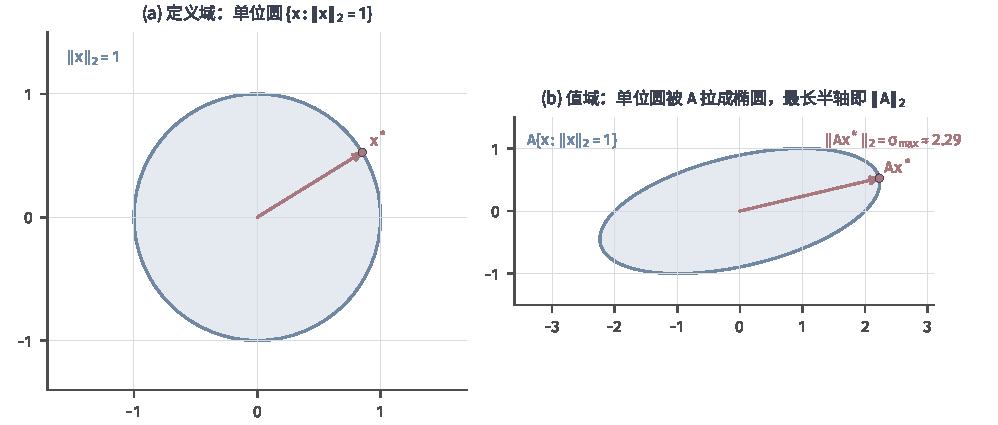
\includegraphics[width=169mm]{figures/01-mathematical-preliminaries-upper/03-linear-spaces/matplotlib/ls-induced-norm-action/ls-induced-norm-action.pdf}
  \caption{诱导矩阵范数衡量最坏放大倍数。左：单位圆$\lVert\bm x\rVert_2=1$；中：同一线性作用$\bm A$把单位圆映成椭圆；右：椭圆上最长的轴给出$\lVert\bm A\rVert_2=\max_{\lVert\bm x\rVert_2=1}\lVert\bm A\bm x\rVert_2$，箭头指示最大放大方向。数值由$\bm A$的教学构造直接得到，是解析例。}
  \label{fig:ls-induced-norm-action}
\end{figure*}

\subsubsection{行列式}
\phantomsection
\label{sec:ls-exterior-determinants}
\label{sec:linear-algebra-scalar-readouts}

一张方阵把单位正方形变成平行四边形、把单位立方体变成平行多面体时，面积或体积放大多少倍？平行四边形的面积不能由两条边的长度直接算出，它还取决于两个向量的相对方向；若再记录定向，交换两个向量的次序会使有向面积变号。下面先建立记录有向体积的外积，再由它得到行列式和它的计算公式。

\paragraph{外积}
对$\mathbb R^d$中的$k$个向量$\bm v_1,\ldots,\bm v_k$，它们的\term{外积}（exterior product，又称\term{楔积}wedge product）$\bm v_1\wedge\cdots\wedge\bm v_k$按两条规则计算。
\begin{itemize}
 \item 多线性：对每个因子分别保持线性组合，即把某个$\bm v_i$换成$a\bm u+b\bm w$时，整个楔积等于$a(\cdots\wedge\bm u\wedge\cdots)+b(\cdots\wedge\bm w\wedge\cdots)$，其余因子不动。
 \item 交替性：交换相邻两个因子，楔积变号，
 \[
  \cdots\wedge\bm v_i\wedge\bm v_j\wedge\cdots
  =-\cdots\wedge\bm v_j\wedge\bm v_i\wedge\cdots.
 \]
\end{itemize}

两条规则先给出两个推论。第一，含有两个相同因子的楔积为零：两个相同因子相邻时，交换它们不改变楔积，却使它变号，所以它等于自身的相反数，只能为零；两个相同因子不相邻时，先用相邻交换把它们移到一起，只改变符号，结论不变。第二，若某个因子是其余因子的线性组合，把这个因子按组合代入并由多线性展开，每一项都含有两个相同因子，所以整个楔积为零。

由此可以确定楔积的一般形状。设$v_{j,i}$是$\bm v_j$的第$i$个坐标，把每个$\bm v_j=\sum_i v_{j,i}\bm e_i$代入并展开，含重复下标的项为零；其余各项按交替性把下标排成递增次序，只改变符号。所以每个楔积都是基楔积$\bm e_{i_1}\wedge\cdots\wedge\bm e_{i_k}$（$i_1<\cdots<i_k$）的线性组合，这样的基楔积共有$\binom{d}{k}$个。$k>d$时，每一项都必然含有重复下标，所以楔积恒为零。

对$\{1,\ldots,k\}$上的一般排列$\pi$，可以反复交换相邻的两个因子，把$\bm v_{\pi(1)}\wedge\cdots\wedge\bm v_{\pi(k)}$排回$\bm v_1\wedge\cdots\wedge\bm v_k$。记$N(\pi)$为$\pi$的逆序对数，即满足$i<j$而$\pi(i)>\pi(j)$的索引对数。每次交换一对相邻且次序颠倒的因子，逆序对数恰好减少$1$，所以恰好经过$N(\pi)$次交换就排好，每次交换变号一次，得到
\[
 \bm v_{\pi(1)}\wedge\cdots\wedge\bm v_{\pi(k)}
 =\operatorname{sgn}(\pi)\,\bm v_1\wedge\cdots\wedge\bm v_k,
 \qquad
 \operatorname{sgn}(\pi)=(-1)^{N(\pi)}.
\]

\paragraph{有向面积与有向体积}
在$\mathbb R^2$中按两条规则展开，
\[
 \bm u\wedge\bm v
 =(u_1\bm e_1+u_2\bm e_2)\wedge(v_1\bm e_1+v_2\bm e_2)
 =(u_1v_2-u_2v_1)\,\bm e_1\wedge\bm e_2,
\]
其中用到$\bm e_1\wedge\bm e_1=\bm e_2\wedge\bm e_2=0$与$\bm e_2\wedge\bm e_1=-\bm e_1\wedge\bm e_2$。系数$u_1v_2-u_2v_1$是$\bm u,\bm v$张成的平行四边形的有向面积：绝对值是面积，符号是定向。

下面用三组向量观察有向面积的数值与符号。
\begin{example}[平面上的有向面积]
\label{ex:ls-oriented-area}
给定：三组有序向量对：$\bm u=(1,0)^\top$与$\bm v=(1,1)^\top$；交换次序后的$\bm v$与$\bm u$；共线的$(1,1)^\top$与$(2,2)^\top$。
计算：按系数公式$u_1v_2-u_2v_1$，三组依次得到
\[
 1\cdot1-0\cdot1=1,\qquad
 1\cdot0-1\cdot1=-1,\qquad
 1\cdot2-1\cdot2=0.
\]
结论：第一组张成面积为$1$的平行四边形；交换次序后面积不变而定向翻转，所以符号变负；共线的两个向量张成的平行四边形退化成线段，有向面积为$0$。
\end{example}
由上面的计数，$\mathbb R^3$中三个向量的楔积只是基楔积$\bm e_1\wedge\bm e_2\wedge\bm e_3$的倍数。这个系数的绝对值是三个向量张成的平行六面体的体积，带符号时称为\term{有向体积}。

\paragraph{行列式的定义}
在$\mathbb R^d$中取$d$个向量，最高阶楔积只剩一个基楔积$\bm e_1\wedge\cdots\wedge\bm e_d$。对$d$阶方阵$\bm A$，把它的各列$\bm A\bm e_1,\ldots,\bm A\bm e_d$作楔积，
\[
 \bm A\bm e_1\wedge\cdots\wedge\bm A\bm e_d
 =(\det\bm A)\,\bm e_1\wedge\cdots\wedge\bm e_d,
\]
标量$\det\bm A$称为\term{行列式}（determinant）。它是$\bm A$把单位立方体变成平行多面体时的有向体积倍数，绝对值为体积比，符号表示定向是否翻转。图~\ref{fig:ls-determinant-oriented-volume}在平面上画出这一缩放。
\begin{figure*}[htbp]
  \centering
  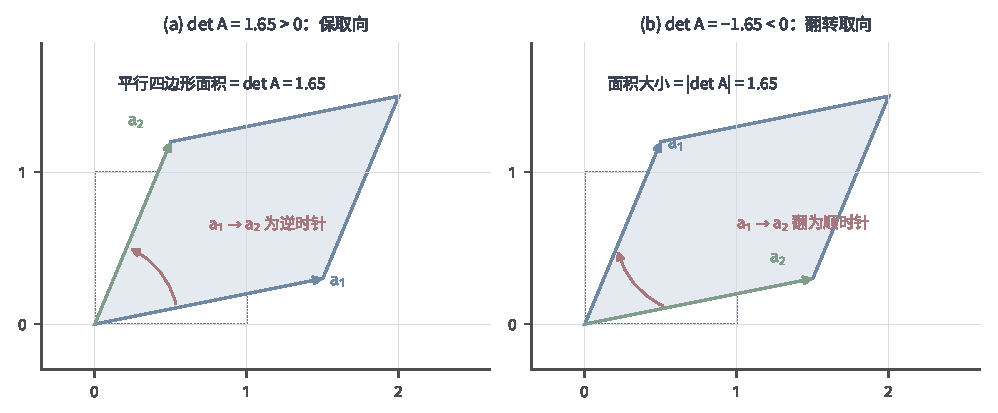
\includegraphics[width=169mm]{figures/01-mathematical-preliminaries-upper/03-linear-spaces/matplotlib/ls-determinant-oriented-volume/ls-determinant-oriented-volume.pdf}
  \caption{行列式作为有向体积的缩放。左：单位正方形由$\bm e_1=(1,0)$、$\bm e_2=(0,1)$张成，面积为$1$。中：$\bm A=\bigl(\begin{smallmatrix}2&0.5\\0&1.5\end{smallmatrix}\bigr)$把它映成由$\bm A\bm e_1=(2,0)$、$\bm A\bm e_2=(0.5,1.5)$张成的平行四边形，有向面积为$2\cdot1.5-0.5\cdot0=3=\det\bm A>0$（保定向）。右：$\bm A$把$\bm e_1$反射到$(-2,0)$，有向面积为$-3$（反定向）。向量与数值均为解析教学例。}
  \label{fig:ls-determinant-oriented-volume}
\end{figure*}

\paragraph{排列展开}
把$\bm A\bm e_j=\sum_i a_{i,j}\bm e_i$代入楔积并展开。若第$j$个因子选出$\bm e_{\tau(j)}$，得到的项为$\bigl(\prod_ja_{\tau(j),j}\bigr)\,\bm e_{\tau(1)}\wedge\cdots\wedge\bm e_{\tau(d)}$。下标有重复的项为零；留下的项中$\tau$是$\{1,\ldots,d\}$的一个排列，而$\bm e_{\tau(1)}\wedge\cdots\wedge\bm e_{\tau(d)}=\operatorname{sgn}(\tau)\,\bm e_1\wedge\cdots\wedge\bm e_d$。所以
\[
 \det\bm A=\sum_{\tau}\operatorname{sgn}(\tau)\prod_{j=1}^d a_{\tau(j),j},
\]
求和遍历全部排列。习惯上按行书写：记$\pi=\tau^{-1}$，把乘积按行号重排，得到$\prod_ia_{i,\pi(i)}$。$\tau$的逆序对$(i,j)$与$\pi$的逆序对$(\tau(j),\tau(i))$一一对应，所以$\operatorname{sgn}(\pi)=\operatorname{sgn}(\tau)$。于是得到计算公式
\[
 \det\bm A
 =\sum_{\pi\in S_d}\operatorname{sgn}(\pi)
   \prod_{i=1}^d a_{i,\pi(i)},
\]
其中$S_d$是$\{1,\ldots,d\}$到自身的全部双射，每个$\pi$规定第$i$行选取第$\pi(i)$列。计算步骤是：对每个排列，从每行各取一个元素、各列恰好取一次，把取出的$d$个数相乘，再按逆序对数的奇偶加上正负号求和。

二阶时只有两个排列：恒等排列没有逆序对，取正号；交换$1,2$的排列有一个逆序对，取负号。于是
\[
 \det\begin{pmatrix}a&b\\c&d\end{pmatrix}=ad-bc,
\]
例如$\det\left(\begin{smallmatrix}1&2\\3&4\end{smallmatrix}\right)=1\cdot4-2\cdot3=-2$。

三阶时有六个排列。恒等排列与两个循环排列$(\pi(1),\pi(2),\pi(3))=(2,3,1)$、$(3,1,2)$的逆序对数为$0$或$2$，取正号；只交换两个位置的三个排列$(1,3,2)$、$(2,1,3)$、$(3,2,1)$的逆序对数为$1$或$3$，取负号。于是
\[
 \begin{aligned}
 \det\bm A={}&a_{1,1}a_{2,2}a_{3,3}+a_{1,2}a_{2,3}a_{3,1}+a_{1,3}a_{2,1}a_{3,2}\\
 &-a_{1,1}a_{2,3}a_{3,2}-a_{1,2}a_{2,1}a_{3,3}-a_{1,3}a_{2,2}a_{3,1}.
 \end{aligned}
\]
下面用这个公式计算一个具体的三阶行列式。
\begin{example}[三阶行列式的排列展开]
\label{ex:ls-det-three-by-three}
给定：$\bm A=\left(\begin{smallmatrix}2&0&1\\1&3&0\\0&1&1\end{smallmatrix}\right)$。
计算：按上式的六项次序代入，
\[
 \begin{aligned}
 \det\bm A&=2\cdot3\cdot1+0\cdot0\cdot0+1\cdot1\cdot1-2\cdot0\cdot1-0\cdot1\cdot1-1\cdot3\cdot0\\
 &=6+0+1-0-0-0=7.
 \end{aligned}
\]
结论：$\det\bm A=7$。六项中只有两项非零，其余四项都含有零元素。
\end{example}

行列式因而是矩阵元素的多项式。上面的推导只说明：若楔积满足两条规则，行列式只能是这个和。反过来可以直接验证，排列展开式作为各列的函数确实对每列线性、交换两列时变号（交换两列相当于把每个$\pi$复合上一次对换，逆序对数的奇偶随之改变），并且在单位矩阵处等于$1$。所以两条规则彼此相容，行列式由它们和$\det\bm I_d=1$唯一确定。高阶时排列有$d!$个，实际计算改用下一小节的性质。

到这里，矩阵的运算都已定义。迹与行列式是方阵的两种不同的标量读取：同一个$\left(\begin{smallmatrix}1&2\\3&4\end{smallmatrix}\right)$迹为$5$而行列式为$-2$。下一小节逐一检查各运算满足的规则。
